\cleardoublepage\chapter{State of the Art}\label{sec:sota}\minitoc\vspace{.5cm}\index{SotA}

\section{Introduction}

\begin{wrapfigure}{r}{0.2\textwidth}
    \centering
    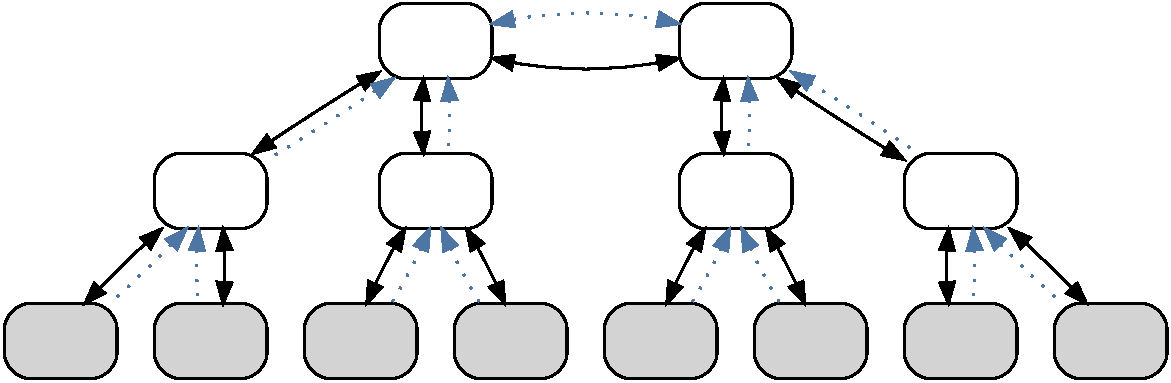
\includegraphics[width=0.2\textwidth]{resources/images/example3}
\end{wrapfigure}

\sidenote{Overview}
\todomid{write}

\section{Related Area 1}\index{Related Area}

\begin{figure}[H]
    \centering
    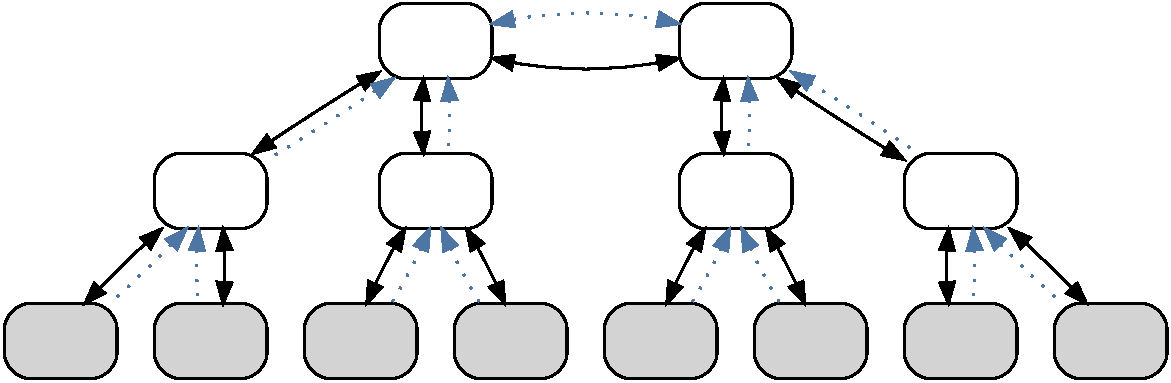
\includegraphics[width=.55\textwidth]{resources/images/example3}
    \caption{Related area 1 within the structure of research}\label{fig:hourglass:ra1}
\end{figure}

\sidenote{Overview}
\todomid{write about \Cref{fig:hourglass:ra1}}

\sidenote{Focus}
\todomid{write}

\subsection{Specific Example 1}

\sidenote{Definition}
\todomid{write}

\sidenote{Issues}
\todomid{write}

\subsection{Specific Example 2}

\sidenote{Definition}
\todomid{write}

\sidenote{Implementations}
\todomid{write}

\sidenote{Research}
\todomid{write}

\sidenote{Standards}
\todomid{write}

\sidenote{Adoption}
\todomid{write}

\subsection{Specific Example 3}\index{Example 3}

\sidenote{Transition}
\todomid{write about \Cref{fig:sota:trans}}

\begin{figure}
    \centering
    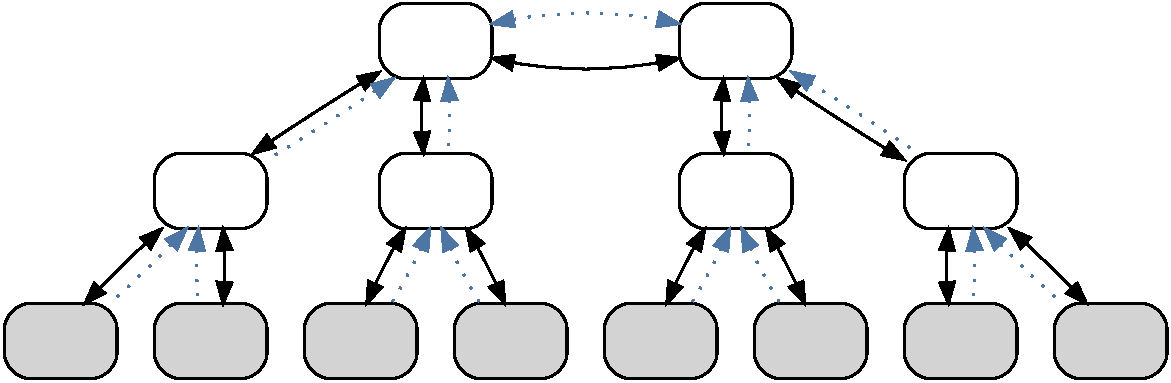
\includegraphics[width=.85\textwidth]{resources/images/example3}
    \caption{Comparison of Example 2 and Example 3 (based on~\cite{li2002design})}\label{fig:sota:trans}
\end{figure}

\sidenote{Standards}
\todomid{write}

\sidenote{Extension}
\todomid{write}

\sidenote{Other Standards}
\todomid{write}

\sidenote{Something}
\todomid{write}

\sidenote{Something}
\todomid{write}

\sidenote{Something}
\todomid{write}

\sidenote{Something}
\todomid{write}

\sidenote{Something}
\todomid{write}

\sidenote{Something}
\todomid{write}

\section{Related Area 2}\index{Related Area 2}

\sidenote{Overview}
\todomid{write}

\sidenote{Focus}
\todomid{write about \Cref{fig:sota:ra2}}

\begin{figure}[!hbtp]
    \centering
    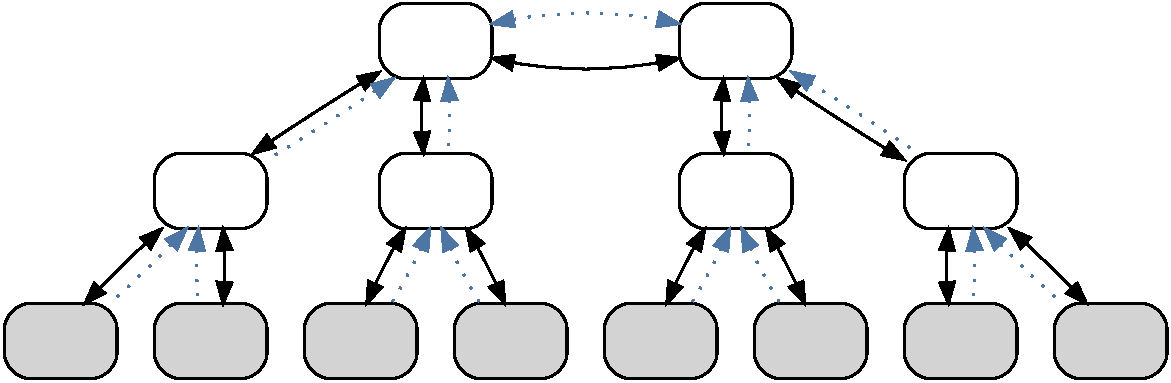
\includegraphics[width=1\textwidth]{resources/images/example3}
    \caption{Related Area 2}\label{fig:sota:ra2}
\end{figure}

\sidenote{Something}
\todomid{write}

\subsection{Specific Example 1}

\sidenote{Definition}
\todomid{write}

\sidenote{Issues}
\todomid{write}

\subsection{Specific Example 2}

\sidenote{Definition}
\todomid{write}

\sidenote{Implementations}
\todomid{write}

\sidenote{Research}
\todomid{write}

\sidenote{Standards}
\todomid{write}

\sidenote{Adoption}
\todomid{write}


\section{Related Area 3}\index{Related Area 3}

\sidenote{Overview}
\todomid{write}

\sidenote{Focus}
\todomid{write about \Cref{fig:sota:ra3}}

\begin{figure}[!hbtp]
    \centering
    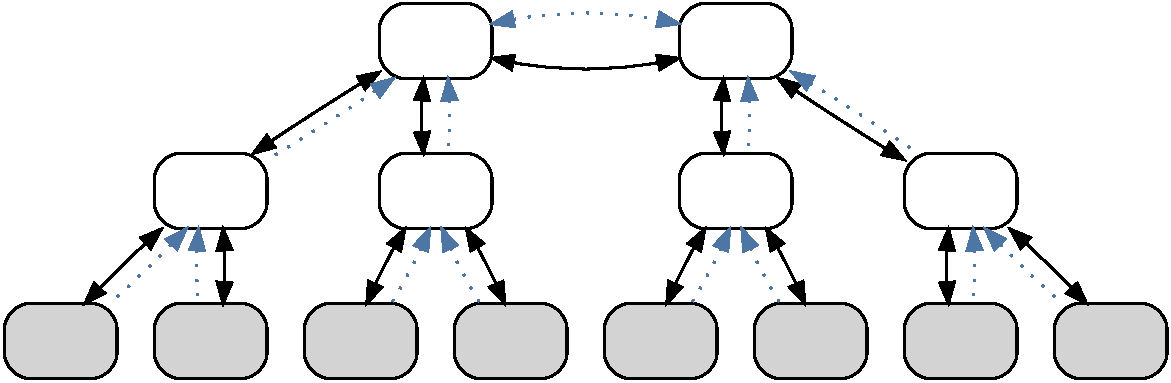
\includegraphics[width=1\textwidth]{resources/images/example3}
    \caption{Related Area 3}\label{fig:sota:ra3}
\end{figure}

\sidenote{Something}
\todomid{write}

\subsection{Specific Example 1}

\sidenote{Definition}
\todomid{write}

\sidenote{Issues}
\todomid{write}

\subsection{Specific Example 2}

\sidenote{Definition}
\todomid{write}

\sidenote{Implementations}
\todomid{write}

\sidenote{Research}
\todomid{write}

\sidenote{Standards}
\todomid{write}

\sidenote{Adoption}
\todomid{write}

\section{Conclusion}

\sidenote{Summary}
\todomid{write}

\sidenote{Takeaway 1}
\todomid{write}

\sidenote{Takeaway 2}
\todomid{write}

\sidenote{Takeaway 3}
\todomid{write}

\sidenote{Next chapter}
\todomid{write}
